% 阶段报告三：中文正式版。编译：xelatex stage_report_3_zh.tex（两遍）。
% 数字来源及独立核验见本目录 verified_numbers.json 和 README.md。
\documentclass[11pt,a4paper,UTF8,fontset=fandol]{ctexart}
\usepackage[margin=0.9in]{geometry}
\usepackage{amsmath,amssymb,booktabs,tabularx,array,graphicx,xcolor,float}
\usepackage[hidelinks]{hyperref}
\usepackage{enumitem}
\setlist{itemsep=3pt,topsep=5pt}
\renewcommand{\refname}{参考文献}
\newcolumntype{Y}{>{\raggedright\arraybackslash}X}
\newcommand{\code}[1]{\nolinkurl{#1}}
\emergencystretch=3em
\linespread{1.15}
\setlength{\parindent}{2em}
\setlength{\parskip}{0pt}
\title{\bfseries 细胞核实例分割中的跨尺度候选筛选与面积过滤\\[7pt]
\large PanNuke 细胞核实例分割：阶段报告三}
\author{课程项目 bdd26}
\date{2026 年 10 月 6 日修订\\\small 实验范围：2026 年 10 月 2 日至 5 日}
\begin{document}
\maketitle

\begin{abstract}
提高工作分辨率有助于检出 PanNuke 数据集中部分死亡核（Dead 类），但也会引入误报，降低整体分割质量。针对这一问题，本阶段在修正后处理实现和历史种子统计的基础上，研究跨尺度候选筛选方法：保留原尺度模型经后处理的预测，仅补入与其不重叠且通过筛选的两倍尺度候选，记为 P2。三个数据划分、每划分三个随机种子的配对实验中，P2 的 Dead 类全景质量（Dead PQ）八组提高、一组不变，但类别无关全景质量（bPQ）的平均损失超过预设接受范围。验证集候选分析发现，类型置信度不足以判断实例是否可靠，面积小于 30 个原始网格像素的新增候选仅有 19.79\% 能与标注匹配。据此，在固定 P2 参数的条件下，引入由验证集选择的面积过滤步骤，得到 EF-P2。

相对同种子的原尺度后处理基线，EF-P2 的 Dead PQ 均值由 0.17255 提高至 0.17954，保留了 P2 原有得分增益的 94.3\%；平均全景质量（mPQ）提高 0.00068，bPQ 平均差值为 $-0.000009$。该方案通过预注册判定规则，表明面积过滤能够在本组实验中减小候选添加带来的整体分割损失。不过，mPQ 和 bPQ 的差值置信区间仍跨零，更严格计入缺类误报的总体指标略有下降，且测试数据已在多轮研究中使用。因此，EF-P2 仍是待独立验证的候选方法，现有结果不足以证明其全面优于基线或具有统计意义上的非劣性，完整推理成本也有待测量。
\end{abstract}
\noindent\textbf{关键词：}细胞核实例分割；PanNuke；尺度互补；候选过滤；配对验证

\section{研究背景与目标}

细胞核实例分割与分类需要同时确定单个细胞核的边界和类别，是病理图像分析的基础任务。PanNuke 数据集包含五类细胞核标注\cite{pannuke}。其中，Dead 类涉及死亡、凋亡及相关碎裂核形态，样本较少，检测和分类均较困难。本文沿用数据集类别名 Dead，不将模型输出解释为病理诊断。

前两阶段分别完成了基线复现、语言辅助分型、合成增强与反事实压力测试，并进一步研究了公开模型和两倍工作分辨率对 Dead 漏检的影响\cite{reports}。已有结果显示，两倍工作尺度模型可以检出部分原尺度模型未能检出的核，但直接替换原尺度预测会降低整体分割质量。本阶段据此研究：能否保留原尺度预测，仅利用两种尺度之间的互补信息补充漏检核，并控制新增误报？

围绕这一问题，本阶段完成了以下工作。
\begin{enumerate}
\item 修正后处理实现，为两种尺度模型设置相同的验证集调参流程，并核对历史实验的种子覆盖情况。
\item 补齐缺失训练，在九个不同的划分--种子组合上进行配对验证，考察跨尺度候选添加的收益及其整体分割代价。
\item 分别分析新增候选的实例匹配情况和分型准确性，依据验证集观察设计面积过滤，并按预先规定的规则评估过滤后的结果。
\end{enumerate}

本阶段的方法建立在既有模型预测之上，不涉及新网络架构，也不以解决全部 Dead 漏检为结论。前两份报告保留为历史记录；旧后处理和种子统计的更正以本报告及 10 月 2 日的审计结果为准\cite{p0p3}。

\section{评测口径与历史更正}

\subsection{数据划分、模型与指标}

本阶段采用以 UNI\cite{uni} 为编码器的 CellViT\cite{cellvit}（CellViT-UNI）。记原尺度模型为 x1，两倍工作尺度模型为 x2，两者分别在相应尺度下训练。M/S 是小面积边界实例删除与同类相邻实例合并的后处理流程，x1+M/S 表示原尺度模型经验证集选择的后处理结果。

实验沿用仓库登记的 PanNuke 三划分协议（表~\ref{tab:splits}）。两种尺度均训练 130 轮，批大小为 16，采用 AdamW 优化器，初始学习率为 $3\times10^{-4}$，权重衰减为 $10^{-4}$，动量参数为 $(0.85,0.95)$；学习率逐轮乘以 0.85，编码器在前 25 轮冻结。18 个模型的保存配置均与各自固定清单一致。自行训练的模型统一使用训练结束时的最终检查点，不根据测试结果选择中间检查点；本阶段主表均不使用测试时增强（test-time augmentation，TTA）。参数仅在对应验证折选择，固定后再应用于测试折。所有正式评测均使用 \code{nucseg.metrics.pannuke_eval}。为对应实验记录，下文将后处理公平对照、尺度互补分析、候选添加和尺度交叉实验分别记为 P0、P1、P2 和 P3。

\begin{table}[H]
\centering\small
\caption{本项目的三划分协议。split 1 与 split 2 共享测试 fold 3，不能当成两批独立病例。}
\label{tab:splits}
\begin{tabular}{lccc}\toprule
划分 & 训练折 & 验证折 & 测试折\\\midrule
split 1 & fold 1 & fold 2 & fold 3\\
split 2 & fold 2 & fold 1 & fold 3\\
split 3 & fold 3 & fold 2 & fold 1\\\bottomrule
\end{tabular}
\end{table}

\begin{table}[H]
\centering\small
\caption{本报告使用的指标。除另有说明，数值范围均为 0--1，越高越好。}
\begin{tabularx}{\linewidth}{lY}\toprule
指标 & 含义及注意事项\\\midrule
mPQ & 同时考虑实例分割与类型，按官方的图像、类别和组织聚合口径计算。\\
bPQ & 忽略核的类型，衡量实例检出与分割质量；不能单独解释为轮廓精度。\\
Dead PQ & 只看 Dead 类；官方口径不计入真值中没有该类的图像。\\
strict Dead PQ & 对没有 Dead 真值、却预测出 Dead 的图像也计罚，补充检查误报。\\
strict mPQ & 将上述更严格的缺类误报处理扩展到总体指标。\\
mPQ$^+$ & 在数据集内按类汇总实例匹配统计的补充指标；仍受类型预测影响，并非纯分割分数。\\\bottomrule
\end{tabularx}
\end{table}

全景质量（panoptic quality，PQ）同时衡量实例检出和掩码重合程度\cite{pq}：
\begin{equation}
\mathrm{PQ}=\frac{\sum_{(g,p)\in\mathrm{TP}}\operatorname{IoU}(g,p)}{|\mathrm{TP}|+\tfrac12|\mathrm{FP}|+\tfrac12|\mathrm{FN}|}\text{。}
\end{equation}
其中，交并比（intersection over union，IoU）为两掩码交集面积与并集面积之比；TP 为 IoU$>0.5$ 的匹配实例对，FP 和 FN 分别为未匹配的预测实例和真值实例。mPQ 和 Dead PQ 在同一类别内建立匹配；bPQ 则忽略类别。候选分析中的“匹配”另指忽略类别、按 IoU$>0.5$ 建立的实例对应关系，“匹配且分型正确”还要求预测类别与真值一致，不能与逐类 PQ 的匹配口径混用。

表中的 $\Delta$ 均表示方法相对同划分、同种子基线的绝对差值。例如 $+0.00699$ 相当于百分制下增加 0.699 分，而非相对提高 0.699\%。下文“九组均值”均先对各划分内的三个种子取平均，再对三个划分取平均；种子数相等时，该值等于九组配对结果的等权均值。

\subsection{历史结果更正}

10 月 2 日的审计发现，旧 M/S 代码存在实例类别索引、周长计算、横纵共享边界累加等问题；验证扫描还曾从合并后的实例/类型图重建真值通道，丢失了官方标注中跨类别重叠的信息。修复后必须重新做验证选择和测试评测，不能只改代码而保留旧分数。v2 保持参数配置集合不变，重跑了受影响的 CPU 阶段。

同时，旧 x2 的 split 2 三个目录实际对应种子 \{19,1,1\}，而非 \{19,1,2\}；当时 x1 也仅在 split 1 有三个种子。目录数量不能代替种子覆盖。因此，旧报告中的“完整 $3\times3$ 种子网格”不成立。本阶段新增四次 x1 训练和一次 x2 训练，才补齐两种尺度下的九个匹配对。

此外，既有结果的解释应限定于已测试的方案：增强实验无效不能推广为所有数据干预均无效，公开模型复评未改善 Dead 也不能否定整个架构家族。检测不足与分型错误可以同时存在。公开的验证集选优权重与本项目自训的最终检查点采用不同的模型选择方式，即使使用相同评测器，也不构成完全一致的实验协议。

\section{尺度互补性与对照实验}

\subsection{P0：不同工作尺度的公平对照}

x1 以 $256\times256$ 为工作网格，x2 将同一图像插值至 $512\times512$。插值不增加新的光学信息，而是改变模型处理纹理和目标的尺度。两倍解码尺度配置记为 du2，仅调整两项解码常数：最小面积由 10 增至 40，Sobel 窗口由 21 增至 41；标记生成中的形态学开运算核保持默认大小，并非全部解码参数均按尺度放大。

M/S 先删除面积低于阈值且接触图像边缘的实例，再合并共享边界足够长的同类相邻实例。横纵接触均按四邻域累计，合并关系由原始实例几何确定。x1 与 x2 分别在验证集上选参数；x1+M/S 是后续融合的公平基线。

\begin{table}[H]
\centering\small
\caption{修正后的尺度对照，仅 seed 19 的三个划分均值。此表用于承接历史，不与后文九对均值混用。}
\label{tab:p0}
\begin{tabular}{lrrrrr}\toprule
配置 & mPQ & bPQ & mPQ$^+$ & Dead PQ & strict Dead PQ\\\midrule
x1 & 0.49951 & 0.66535 & 0.51781 & 0.17601 & 0.13299\\
x1+M/S & 0.49983 & 0.66562 & 0.51746 & 0.17669 & 0.13405\\
x2+du2 & 0.48938 & 0.65827 & 0.51573 & 0.18311 & 0.12139\\
x2+du2+M/S & 0.49058 & 0.66009 & 0.51502 & 0.18499 & 0.12493\\\bottomrule
\end{tabular}
\end{table}

表~\ref{tab:p0} 中，M/S 也能改善 x1 的 mPQ 和 bPQ 均值，并非 x2 独有的优势。直接采用 x2+du2+M/S，官方 Dead PQ 较高，strict Dead PQ 却较低。这提示我们：多检出的核和新增误报必须同时检查，不能只挑有利的 Dead 口径。

\subsection{P1：实例互补性与类型交换分析}

P1 对原始 x1 与修正后的 x2+du2+M/S 做实例级比较。内部 Dead 指合并真值实例图中不接触图像任意一条边的 Dead 核；只要有一个像素接触四边之一，即归为贴边实例。测试集内部 Dead 的类别无关匹配率，按三个划分分别计算再平均，从 53.27\% 升至 60.00\%。但验证集与 x1 完全不重叠的 x2 候选中，只有约 30\% 能同时满足匹配和分型正确。

固定掩码，仅在稳定的一对一配对实例间交换类型后，保留 x2 掩码、采用 x1 类型的 mPQ 由 0.49058 提高至 0.49740；反向交换则使 x1 的 mPQ 由 0.49951 降至 0.49253。这说明稳定配对实例的类型差异与部分性能差距有关，但不构成针对全部实例的分类因果分解。由于掩码不变，bPQ 不受类型交换影响。

P1 还使用真值筛选候选，检查“只补入正确候选”可能获得多少收益。这类真值辅助实验仅用于诊断，不是可部署方法，更不是所有融合方法的数学上界。实际 P2 不使用真值决定测试时添加什么。

\subsection{P3：训练与推理尺度交叉实验}

在 split 1 的固定 128 张验证图上，将训练尺度与推理尺度交叉，得到表~\ref{tab:p3}。这批图含 3,693 个真值核，其中 84 个 Dead 分布在 11 张图中。

\begin{table}[H]
\centering\small
\caption{P3 机制探查：同一验证子集，推理尺度与解码尺度同步变化。不是完整测试结果。}
\label{tab:p3}
\begin{tabular}{ccrrr}\toprule
训练网格 & 推理网格 & mPQ & bPQ & Dead PQ\\\midrule
256 & 256 & 0.48687 & 0.66423 & 0.12776\\
256 & 512 & 0.30631 & 0.44754 & 0.12322\\
512 & 256 & 0.36747 & 0.55432 & 0.05107\\
512 & 512 & 0.48701 & 0.65484 & 0.25276\\\bottomrule
\end{tabular}
\end{table}

尺度不匹配时整体分数明显下降，说明模型已适应训练时的目标尺度。但该实验没有完全分离编码器、监督目标和解码的影响；Dead 样本也很少。它支持“训练与推理尺度应配套”，不足以单独证明某一网络部件造成了尺度收益。

\section{P2：保留基线预测的跨尺度候选添加}

P2 完整保留 x1+M/S 的实例掩码和类型，只考虑来自\textbf{原始 x2+du2 预测}且与基线没有任何像素重叠的候选。候选以完整实例加入，不裁切、不覆盖、不替换已有实例。概率表须与原始候选实例编号对应；经过合并或重编号的预测不能直接沿用旧概率行。

候选配置在实验前固定：面积上限为 \{100,200\}，类型置信度下限为 \{0.5,0.7,0.9\}，另设是否排除贴边实例，共 12 种组合。此外，设置不添加的恒等配置（identity）和不筛选的诊断对照。所有面积均以还原后的 $256\times256$ 网格上的像素数计，而非像素边长。

置信度取候选最终预测类别对应的平均概率。x2 输入图像经双线性插值放大，在 $512\times512$ 网格上完成预测和解码后，实例图与类型图以最近邻插值还原至 $256\times256$。面积在还原后的网格上统计，类型概率则在 $512\times512$ 候选掩码内取平均，只保留还原后仍存在的实例编号对应的概率行。最终类别由类型图多数票决定，因此该概率未必等于概率表中的最大值；它反映类别判断的置信度，不能直接视为核实例存在的概率。

验证选择同时要求：相对 x1+M/S，mPQ 和 bPQ 均不低于基线减 0.002，strict Dead PQ 不下降，内部 Dead 真值的匹配数增加。在符合条件的配置中，依次按验证 mPQ 降序、添加数升序和配置名称排序选择；若无配置满足条件，则采用 identity。这些条件是验证集点估计的接受门槛，不是统计意义上的非劣性检验。

seed 19 的首轮结果中，split 1 回退到 identity，split 2 和 3 采用添加。三划分平均 Dead PQ 增加 0.00685，bPQ 减少 0.00045，当时只能将其列为待验证候选。

\subsection{类型置信度与实例匹配的关系}

10 月 3 日的分型审计将两个问题分开统计：候选是否与真值核匹配，以及匹配之后类别是否正确。结果见表~\ref{tab:typing}。

\begin{table}[H]
\centering\small
\caption{seed 19 的 P2 测试添加。分型正确率的分母是已匹配候选，不是全部添加。split 1 没有添加。}
\label{tab:typing}
\begin{tabular}{lrrrr}\toprule
划分 & 添加数 & 匹配数 & 匹配率 & 匹配后分型正确率\\\midrule
split 2 & 1,679 & 715 & 42.58\% & 87.55\%\\
split 3 & 2,713 & 1,066 & 39.29\% & 85.83\%\\\bottomrule
\end{tabular}
\end{table}

高置信度筛选确实选出了较容易正确分型的对象，却仍有 57--61\% 的添加不能与真值达到 IoU$>0.5$。这里的“未匹配”既可能来自误检，也可能来自几何偏差或碎片，不能直接断言病理图像中绝对不存在对应结构；但在评测中，它们仍会形成实例误报成本。

Dead 候选的分型准确性在验证集和测试集之间也有差异。对于 split 2 中通过 0.9 概率阈值、预测为 Dead 且已匹配的新增候选，真值同为 Dead 的比例由验证集的 85.04\%（108/127）降至测试集的 66.67\%（62/93）。按相同的预测类别分组，原始 x2 测试预测的对应比例均值为 57.88\%，x1 为 55.39\%。这些比例的分母均不是全部真实 Dead 核，因此不能解释为 Dead 分类召回率，也不足以说明 x2 对全部真实 Dead 的分型更好。它们提示，新增候选的匹配可靠性与匹配后的类型正确性需要分别评估。

\section{P2 的配对验证结果}

本阶段补齐了三个划分、种子 \{19,1,2\} 下的 x1/x2 组合。每个匹配对分别做 P0 和 P2 验证选择；全部 18 份选择冻结后才开始本轮测试应用。不同种子可能选到不同参数，这是同一验证选择流程的重复，而非强迫所有模型使用 seed 19 的参数\cite{matchedplan}。

预注册规则如下。对每个指标，先计算各划分内三个种子的配对差值，再求均值与总体标准差（\code{ddof=0}）。取三个划分中最大的差值标准差为 $s_{\max}$。只有同时满足以下条件，才标记为通过：
\begin{enumerate}
\item Dead PQ 的九组配对均值增量不小于其 $s_{\max}$；
\item 九个匹配对中至少七对 Dead PQ 不下降；
\item mPQ、bPQ 的平均差值分别不低于各自的 $-s_{\max}$。
\end{enumerate}

这是一套事先约定的接受标准，不是常规显著性检验，也不是预先给定临床容忍量的非劣性设计。这里的标准差来自\textbf{配对差值}，不能替换成原始模型分数的种子标准差。

P2 的 Dead PQ 平均增加 0.00742，大于最大配对差值标准差 0.00312；八对提高，一对 identity 不变。但 bPQ 的平均配对差值为 $-0.00087$，低于允许下限 $-0.00064$，因此未通过判定。

损失主要集中在 split 3：其 Dead PQ 平均增加 0.01632，而 bPQ 减少 0.00179；对应的图像 bootstrap 区间分别位于零的正侧和负侧。P2 的优势和代价都能重复出现，不能因 Dead 改善就省略 bPQ 的下降。

M/S 本身的次要对照也比旧报告更温和：九对平均 $\Delta$mPQ 为 $+0.00028$，$\Delta$bPQ 为 $+0.00030$，$\Delta$Dead PQ 为 $+0.00046$；三个指标各有 7/9 对非负。它有小幅平均收益，但不是每一对、每一个划分都改善。

\section{验证集候选分析与面积过滤方法}

\subsection{候选面积与匹配率}

为分析能否通过少量过滤降低新增误报，本阶段仅使用九组配对实验中已经固定的验证集新增候选开展存在性审计。这里的“存在性”以候选能否与标注实例匹配来衡量，不等同于病理学意义上对象是否真实存在。

共统计 17,359 个新增候选，其中 7,204 个与真值匹配，汇总匹配率为 41.50\%。这些记录来自多个模型对重叠图像集的预测，并非 17,359 个独立实例样本或病例。按面积分组后，最小面积组的匹配率最低（表~\ref{tab:area}）。

\begin{table}[H]
\centering\small
\caption{冻结 P2 验证添加的面积分组。面积以原始 256 网格的像素数计，所有分组均来自实际记录。}
\label{tab:area}
\begin{tabular}{lrrrr}\toprule
面积 & 添加数 & 匹配数 & 匹配率 & 匹配且正确分为 Dead\\\midrule
小于 30 & 2,294 & 454 & 19.79\% & 43\\
30--59 & 6,473 & 2,874 & 44.40\% & 354\\
60--99 & 4,976 & 2,435 & 48.93\% & 237\\
100--149 & 2,372 & 1,026 & 43.25\% & 59\\
150--199 & 1,225 & 408 & 33.31\% & 6\\
200 & 19 & 7 & 36.84\% & 0\\\midrule
合计 & 17,359 & 7,204 & 41.50\% & 699\\\bottomrule
\end{tabular}
\end{table}

面积小于 30 的候选占全部新增候选的 13.2\%，仅占全部匹配候选的 6.3\%。但该组仍含 43 个正确匹配并分型的 Dead 候选，说明面积过滤存在误删正确候选的风险。

与基线的有限距离分组中，匹配率约为 39--44\%，不足以支持单按距离过滤。圆度和填充率也有边际差异，但尚未证明它们在控制面积、类别和组织组成后仍有独立价值。没有新增候选重复匹配基线已匹配的真值；这在很大程度上是“预测互不重叠且匹配要求 IoU$>0.5$”的结构约束所致，不是排除了所有碎片机制的额外证据。

\subsection{EF-P2 的候选配置与选择规则}

面积过滤方法记为 EF-P2（existence-filtered P2），仅处理各组已经固定的 P2 新增候选，不改变 x1+M/S 基线或 P2 参数。预注册的候选配置集合包含五项\cite{efplan}：
\begin{itemize}
\item \textbf{identity}：不添加，返回 x1+M/S；
\item \textbf{off}：关闭面积过滤，完整保留 P2 添加；
\item \textbf{a30}：保留面积至少 30 的添加；
\item \textbf{a30d}：非 Dead 添加面积至少 30，预测为 Dead 的添加豁免；
\item \textbf{a60}：保留面积至少 60 的添加。
\end{itemize}

EF 沿用 P2 的验证联合门槛和选择次序。off 必须在 mPQ、bPQ、strict Dead、内部 Dead 匹配数、添加数这五项量上重现冻结 P2 行，容差不超过 $10^{-12}$。九对都通过了检查；这证明第一阶段的选择量被正确复现，不等于单靠这项检查就证明了整个预测文件逐字节相同。

所有九份 EF 验证选择冻结后，再应用到测试折。最终七对选择 a30，split 1/seed 1 选择 a30d，split 1/seed 19 继续 identity。这个结果也说明，方法不是在全体图像上强制使用同一个 30 像素阈值，而是重复同一套验证集选择流程。

\section{EF-P2 的实验结果}

表~\ref{tab:main} 是当前主表。每个划分先平均三个种子，再平均三个划分；由于每个划分种子数相同，这与九对等权均值一致。基线为同种子的 x1+M/S，不是未经后处理的 x1，也不是旧 seed 19 的 0.4995 mPQ。

\begin{table}[H]
\centering\footnotesize
\setlength{\tabcolsep}{3pt}
\caption{九组划分--种子配对实验的测试结果。strict 指标仅报告点估计，未计算对应的 bootstrap 区间；差值由未舍入数值计算。}
\label{tab:main}
\begin{tabular}{lrrrrrr}\toprule
配置 & mPQ & bPQ & mPQ$^+$ & strict mPQ & Dead PQ & strict Dead PQ\\\midrule
x1+M/S & 0.49760 & 0.66530 & 0.51594 & 0.45251 & 0.17255 & 0.13073\\
P2 & 0.49769 & 0.66443 & 0.51905 & 0.45147 & 0.17997 & 0.13363\\
EF-P2 & 0.49828 & 0.66529 & 0.51974 & 0.45221 & 0.17954 & 0.13406\\\midrule
P2 差值 & +0.00008 & -0.00087 & +0.00311 & -0.00104 & +0.00742 & +0.00290\\
EF-P2 差值 & +0.00068 & -0.000009 & +0.00380 & -0.00030 & +0.00699 & +0.00333\\\bottomrule
\end{tabular}
\end{table}

EF-P2 保留了 P2 原有 Dead PQ 增益的 94.3\%，同时将 bPQ 平均损失由 0.00087 减小至约 0.000009。相对未过滤的 P2，八组非 identity 配对的 mPQ、bPQ 均提高，Dead PQ 的变化则有正有负。这与验证集中小面积候选匹配率较低的观察一致，但得分增益保留率不等于正确实例保留率，对被删除候选的组成仍需逐实例核查。

\begin{figure}[H]
\centering
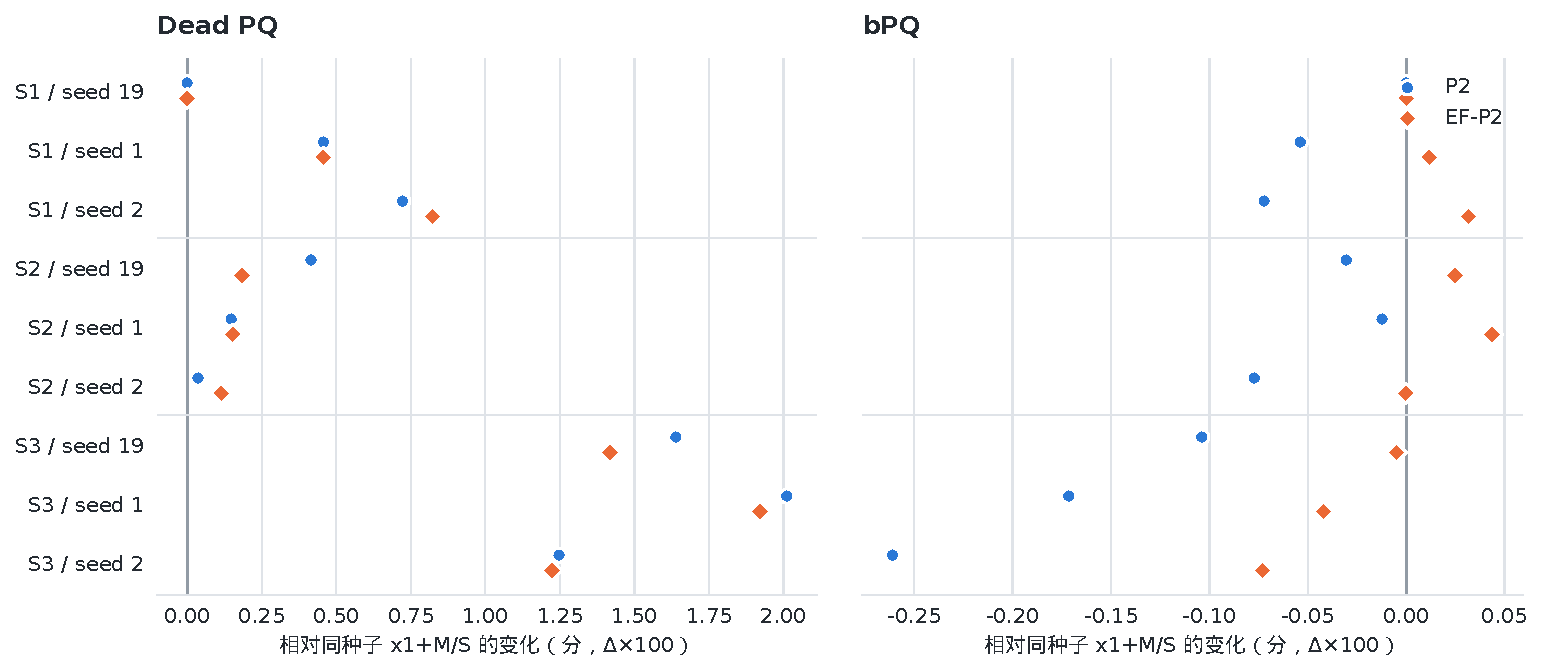
\includegraphics[width=\linewidth]{figs/paired_gains_zh.pdf}
\caption{每个划分--种子对相对自身 x1+M/S 的变化。圆点为 P2，菱形为 EF-P2；图中使用百分制差值（原始 $\Delta\times100$）。Dead 的两种方法均为八对提高、一对不变；bPQ 的 EF-P2 结果更接近零。零差值不计为提高。}
\label{fig:pairs}
\end{figure}

按预注册规则，EF-P2 的 Dead PQ 均值增量 0.00699 大于最大配对差值标准差 0.00337，八组为正、一组为零；mPQ 的平均配对差值为正，bPQ 的平均配对差值也高于下限 $-0.000279$。因此，EF-P2 满足全部接受条件，被保留为后续独立验证的候选方法。该判断仅适用于预注册规则，不替代显著性检验或非劣性检验。

\subsection{不确定性与划分间差异}

每个划分分别进行 2,000 次按组织分层的配对图像 bootstrap，随机种子为 20261004。三个训练种子共享同一组重采样图像索引，再求配对差值均值；不把不同划分混在一起。表~\ref{tab:ci} 和图~\ref{fig:ci} 给出 EF-P2 的结果。

\begin{table}[H]
\centering\small
\caption{EF-P2 减同种子基线：各划分三种子均值及 95\% 配对图像 bootstrap 区间。}
\label{tab:ci}
\begin{tabular}{llrr}\toprule
划分 & 指标 & 均值差 & 95\% 区间\\\midrule
split 1 & mPQ & +0.000653 & [$-0.000324$, $+0.001566$]\\
 & bPQ & +0.000145 & [$-0.000709$, $+0.000944$]\\
 & Dead PQ & +0.004265 & [$+0.000962$, $+0.007959$]\\\midrule
split 2 & mPQ & +0.000445 & [$-0.000317$, $+0.001197$]\\
 & bPQ & +0.000228 & [$-0.000492$, $+0.000880$]\\
 & Dead PQ & +0.001505 & [$-0.000534$, $+0.003594$]\\\midrule
split 3 & mPQ & +0.000944 & [$-0.000462$, $+0.002469$]\\
 & bPQ & $-0.000400$ & [$-0.001567$, $+0.000781$]\\
 & Dead PQ & +0.015204 & [$+0.005719$, $+0.026246$]\\\bottomrule
\end{tabular}
\end{table}

\begin{figure}[H]
\centering
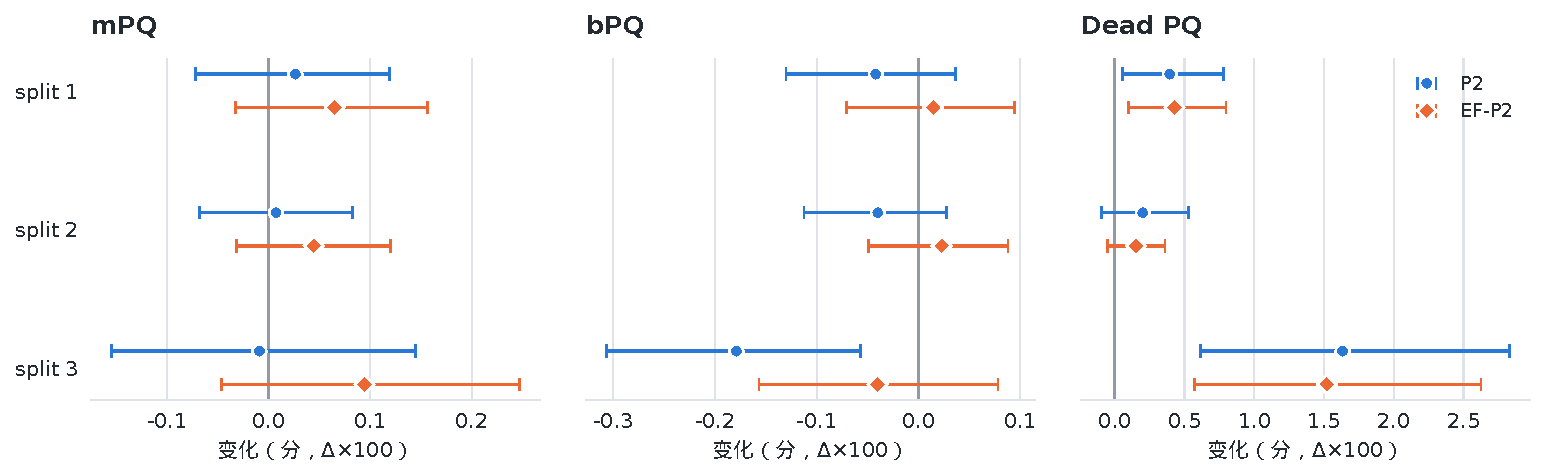
\includegraphics[width=\linewidth]{figs/split_intervals_zh.pdf}
\caption{P2 与 EF-P2 的逐划分区间比较。每个小图有自己的横轴刻度，均为百分制差值。过滤后 split 3 的 bPQ 区间从完全低于零变为跨零；这不等于证明 bPQ 没有损失。Dead 的改善仍以 split 3 最明显。}
\label{fig:ci}
\end{figure}

Dead 在 split 1 和 3 的区间不跨零，split 2 仍跨零；三个划分的 mPQ、bPQ 区间全部跨零。这些区间\textbf{以已训练好的三个种子为条件}，不包含重新训练所带来的全部不确定性。每个划分仅三个种子，标准差本身的估计也不稳定。

更严格的指标还保留了一个警示：EF-P2 的 strict mPQ 平均下降 0.00030，split 2 的 strict Dead PQ 平均下降约 0.00013。整体平均和官方 Dead 口径的改善，并没有消除所有类别或所有划分上的代价。

\section{边界分组的事后复核}

EF 实验完成后，存在性审计的边界分组实现被发现有误：旧表误用了面积分箱，导致贴边与内部两行全为零。修正后，从冻结验证预测重新生成的 v2 表见表~\ref{tab:border}。其他分组与原始记录的既有列未改变，EF 配置集合也不依赖旧边界表，因此九对 EF 分数不受影响。

\begin{table}[H]
\centering\small
\caption{事后重建的边界统计，仅验证添加。贴边指候选接触原始预测图的任意一条边。该表没有用于设计 EF 配置集合。}
\label{tab:border}
\begin{tabular}{lrrrr}\toprule
位置 & 添加数 & 匹配数 & 匹配率 & 匹配且正确分为 Dead\\\midrule
贴边 & 9,975 & 5,273 & 52.86\% & 85\\
内部 & 7,384 & 1,931 & 26.15\% & 614\\\bottomrule
\end{tabular}
\end{table}

这组结果不支持把“贴边”本身当成删除候选的理由：贴边组总体匹配率更高，而正确补回的 Dead 主要在内部。两组的类别、面积和折组成并不相同，不能把差异解释为边界位置的因果效应，也不能据此立即增加一条新过滤规则。当前冻结配置集合保持不变。

同日还修复了 EF 测试入口的 identity 回退分支，现存九组结果未触发该缺陷，具体说明见附录。

\section{讨论与后续工作}

\subsection{研究局限}

本阶段结果支持将面积过滤用于控制跨尺度候选添加的平均分割损失，但仍有以下局限。
\begin{enumerate}
\item \textbf{收益范围有限。}主要收益集中在 Dead 类，整体 mPQ 增量较小，strict mPQ 略有下降；逐划分的 mPQ 和 bPQ 区间均跨零，不能据此证明非劣性。
\item \textbf{测试数据重复使用。}EF-P2 是 P0--P3 v2、配对验证和 EF-P2 三轮中的第三轮预注册测试评测，更早的机制分析也使用过这些图像。轮内仅用验证集选择参数，仍不能消除跨轮研究对既有测试结果的适应。共享测试折也不构成独立病例重复。
\item \textbf{完整成本尚未测量。}面积过滤本身仅需 CPU 计算，但候选生成需要 x1 和 x2 两套模型预测。完整推理时延、峰值资源占用及能耗尚不明确。
\item \textbf{历史来源记录不完整。}旧预测文件未内嵌检查点哈希，部分来源依赖保存配置和配套清单核对。输入文件哈希能够标识固定快照，但不能补充生成时未记录的权重绑定关系。
\item \textbf{缺少独立外部验证。}EF-P2 尚未在独立外部数据或患者级留出数据上验证，也未在现有三个随机种子之外开展重复实验。现有结果不足以支持病理应用有效性或跨数据集泛化能力的结论。
\end{enumerate}

\subsection{后续验证计划}

下一阶段应固定 EF-P2 的配置集合与选择规则，不再依据现有测试图扩展形状阈值、类别阈值或一致性规则。优先在预先确定的独立数据或严格留出设计上比较 x1+M/S、P2 和 EF-P2，并事先约定 Dead 收益、整体损失容忍量和成本指标。若暂不具备独立验证条件，应将本轮结果限定为探索性发现，而不将同源数据上的重复评测视为独立确认。

同时，应测量包含两套模型预测和最终后处理的完整流程，而非只计算面积过滤耗时。定性分析则应采用预先固定的抽样规则，分别展示补回的 Dead、被删除的假阳性、被误删的真阳性和不同划分的失败案例。图像样例用于解释结果，不用于重新选择阈值。

\section{结论}

本阶段在保留原尺度预测的基础上，对两倍工作尺度模型提供的新增候选进行筛选，并进一步引入由验证集选择的面积过滤。九组配对实验中，EF-P2 相对 x1+M/S 的 Dead PQ 平均提高 0.00699，保留了 P2 原有增益的 94.3\%；bPQ 平均差值由 $-0.00087$ 缩小至约 $-0.000009$。这一结果表明，面积过滤可缓解本组实验中候选添加带来的整体分割损失。不过，整体指标差值区间仍跨零，strict mPQ 略有下降，测试数据也已在多轮研究中使用。因此，EF-P2 仍应视为待独立验证的候选方法，其泛化能力与完整推理成本尚需进一步评估。

\appendix
\section{文件、数字与复现入口}

\subsection{数值与实现核验}

本次修订从原始评测汇总中重新提取两轮各九组、六项指标，共 108 个配对差值，与统计文件逐项核对；同时从候选记录重算面积和修正版边界分组。六组逐划分 bootstrap 结果也由逐图统计重新计算，差值区间与存档一致。研究日志\cite{findings}仅用于追溯实验过程，不作为最终数值依据。

2026 年 10 月 6 日，在固定依赖环境下运行完整回归测试，结果为 \textbf{157 项通过，63 条警告}。警告主要涉及依赖弃用及接口提示；本次未安装或升级依赖，也未修改训练、推理及评测实现。另修复制图脚本的中文字体嵌入问题，并新增 PDF 文字提取回归用例。测试通过仅说明现有回归用例通过，不代表全部潜在实现错误均已排除。

EF 的历史回退缺陷为：第一阶段 P2 非 identity、第二阶段 EF 选择 identity 时，未正确取消新增候选。现存九组中唯一的 EF identity 在第一阶段已为 identity，因此原有分数未受影响；当前回归测试已覆盖该组合。历史选择清单的源码指纹保持不变，重跑历史评测须使用匹配快照，或在新输出目录明确登记复核版本，不得绕过来源检查。

\subsection{文件与复现命令}

本报告的可移植文件集中于 \code{docs/report/stage_report_3/}。正式中文、英文和中文导读均提供 TeX 与 PDF；\code{figs/} 保存图表及对应 CSV，\code{verified_numbers.json} 保存主表与存在性统计的核验快照。不在报告中附带模型权重、原始数据、机器配置或凭据。

\begin{table}[H]
\centering\footnotesize
\caption{主要实验产物根目录，均相对 \code{runs/analysis/}。它们是本地实验产物，不随 Git 分发。}
\begin{tabularx}{\linewidth}{lY}\toprule
目录 & 本报告用途\\\midrule
\code{p0p3_20261002_v2/} & seed 19 尺度对照、P1 诊断、P2 首轮与 P3 验证探查。\\
\code{typing_audit_20261003/} & 匹配率、匹配后类型正确率与置信度迁移。\\
\code{matched_seed_20261004/} & 九对 P0/P2 选择、测试评测、差值及 bootstrap。\\
\code{existence_ef_20261005/} & 九对 EF 选择、测试评测与相同口径统计。\\
\code{existence_audit_20261005_v2/} & 重新核验的候选记录、面积与边界分组。\\\bottomrule
\end{tabularx}
\end{table}

在固定依赖环境、仓库根目录执行以下只读提取或制图命令：
\begin{quote}\small
\code{python scripts/report3_numbers.py}\\
\code{python scripts/verify_report3.py}\\
\code{python scripts/make_report_figures3.py}\\
\code{python -m pytest -q}
\end{quote}
核验脚本在缺失必要产物或数值不一致时直接报错，不修改实验结果。\code{report3_numbers.py} 的旧存在性路径仅用于未变化的非边界分组；本报告的边界数字仅来自 v2。重跑历史选择与评测还须使用匹配的源码快照，不能为了通过来源检查而修改冻结清单。

\begin{thebibliography}{9}
\raggedright
\bibitem{pannuke} GAMPER J, ALEMI KOOHBANANI N, BENES K, et al. PanNuke Dataset Extension, Insights and Baselines[EB/OL]. 2020[2026-10-06]. \url{https://arxiv.org/abs/2003.10778}.
\bibitem{reports} bdd26 项目. 阶段报告一、二及 2026-10-02 更正附页[R]. 2026. \code{docs/report/stage_report_1/}; \code{docs/report/stage_report_2/}.
\bibitem{p0p3} bdd26 项目. P0--P3 执行结果与研究判断：v2[R]. 2026-10-02. \code{docs/P0_P3_RESULTS_2026-10-02.md}.
\bibitem{uni} CHEN R J, DING T, LU M Y, et al. Towards a general-purpose foundation model for computational pathology[J]. Nature Medicine, 2024, 30(3): 850--862. DOI: \href{https://doi.org/10.1038/s41591-024-02857-3}{10.1038/s41591-024-02857-3}.
\bibitem{cellvit} H\"ORST F, REMPE M, HEINE L, et al. CellViT: Vision Transformers for precise cell segmentation and classification[J]. Medical Image Analysis, 2024, 94: 103143. DOI: \href{https://doi.org/10.1016/j.media.2024.103143}{10.1016/j.media.2024.103143}.
\bibitem{pq} KIRILLOV A, HE K, GIRSHICK R, et al. Panoptic Segmentation[C]//2019 IEEE/CVF Conference on Computer Vision and Pattern Recognition. 2019: 9396--9405. DOI: \href{https://doi.org/10.1109/CVPR.2019.00963}{10.1109/CVPR.2019.00963}.
\bibitem{matchedplan} bdd26 项目. 匹配种子验证预注册协议：含执行注记[R]. 2026-10-03. \code{docs/superpowers/plans/2026-10-03-matched-seed-validation.md}.
\bibitem{efplan} bdd26 项目. Existence-filtered P2 预注册协议：含事后审计说明[R]. 2026-10-05. \code{docs/superpowers/plans/2026-10-05-existence-filter-p2.md}.
\bibitem{findings} bdd26 项目. 实验日志：2026-10-03 至 10-05 条目[R]. 2026. \code{docs/findings.md}.
\end{thebibliography}
\end{document}
